\problemname{Solnedgång}

Du är på besök i ett varmt land och det råkar vara en stekhet dag, men som tur är befinner du dig i skuggan av ett hus. Du inser att du borde röra dig mot hotellet någon gång, men samtidigt inser du att det är för varmt för att gå ut i solen. Staden som du befinner dig i består av $N$ stycken hus placerade på ett rutnät, varje hus tar upp exakt 1 ruta. Just nu så har alla hus en skugga som är exakt 1 ruta lång och är riktad norrut och då solen har börjat gå ned så ökar längden på denna skugga med 1 ruta per tidsenhet. Du kan gå från skuggan av ett hus till ett annat om skuggorna delar en kant av längd minst 1 (se bild). Du kan inte gå genom hus. Frågan är nu hur lång tid det kommer att ta innan det finns en väg till hotellet som inte involverar brännskador. Hotellet är hus $N$ och du befinner dig i skuggan till hus 1. Då hotellets entré ligger på norra sidan av huset så måste du ta dig till den sidan. I värsta fall så kan du behöva vänta på att det blir natt vilket inträffar efter $K$ tidsenheter.

\begin{figure}[ht!]
\centering
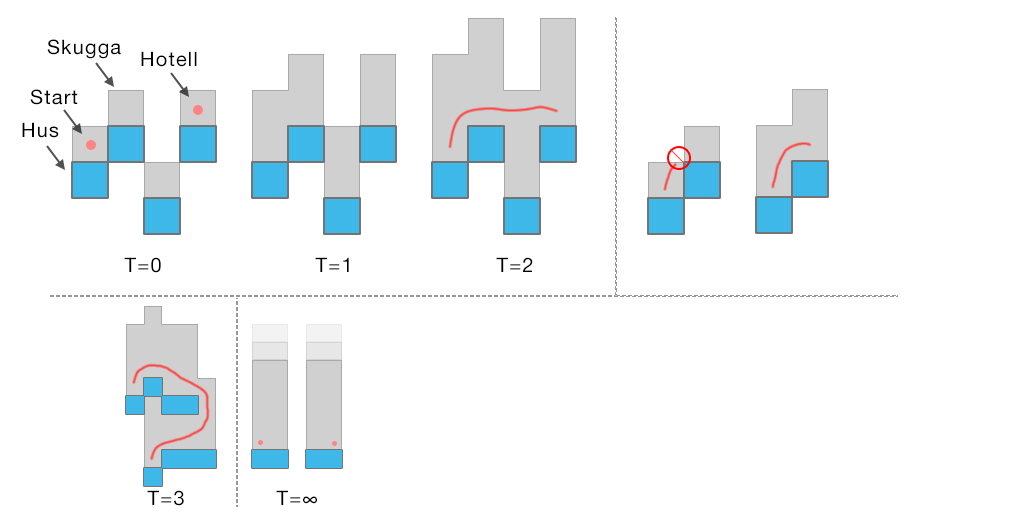
\includegraphics[width=0.6\textwidth]{skuggor.png}
\label{overflow}
\end{figure}

\section*{Input}
På första raden står två heltal $N$ och $K$ antalet hus i staden och antalet tidsenheter innan det blir natt. På de följande $N$ raderna står 2 heltal per rad $x y$, koordinaterna för varje hus. Den första raden har koordinaten vars skugga du står i och den sista raden har koordinaten för hotellet.

Det är garanterat att varje hus har en skugga, dvs inget hus står precis på rutan söder om ett annat hus.

\section*{Output}
Skriv ut ett heltal som motsvarar tiden det tar innan en hel väg till hotellet som endast går genom skuggor existerar eller \texttt{"NATT"} om tiden det skulle ta överskrider eller är lika med $K$.

\section*{Poängsättning}
Din lösning kommer att testas på en mängd testfallsgrupper. För att få poäng för en grupp så måste du klara alla testfall i gruppen.

För alla testgrupper gäller $1 \le N, 0 \le K$.

\begin{tabular}{| l | l | l |}
	\hline
	Grupp & Poängvärde & Begränsningar\\ \hline
	1 & 19 & $N, K \le 100, 0 \le x, y \le 100$ \\ \hline
	2 & 26 & $N, K \le 1000, 0 \le x, y \le 1000$ \\ \hline
	3 & 17 & $N, K \le 1000, 0 \le x, y \le 100000$ \\ \hline
	4 & 23 & $N \le 20000, K \le 10^7, 0 \le x, y \le 10^7$ \\ \hline
	5 & 15 & $N \le 300000, K \le 10^{18}, 0 \le x, y \le 10^{18}$ \\ \hline
\end{tabular}
